%======================================================================
\chapter{Conclusion and Future Work}
\label{ch: Chapter6}
%======================================================================

%----------------------------------------------------------------------
\section{Algorithm Comparison}
%----------------------------------------------------------------------

%----------------------------------------------------------------------
\section{Conclusion}
%----------------------------------------------------------------------

%----------------------------------------------------------------------
\section{Future Work}
%----------------------------------------------------------------------
\subsection{Enhanced Smart Framework}
\begin{figure}[!htbp]
    \centering
    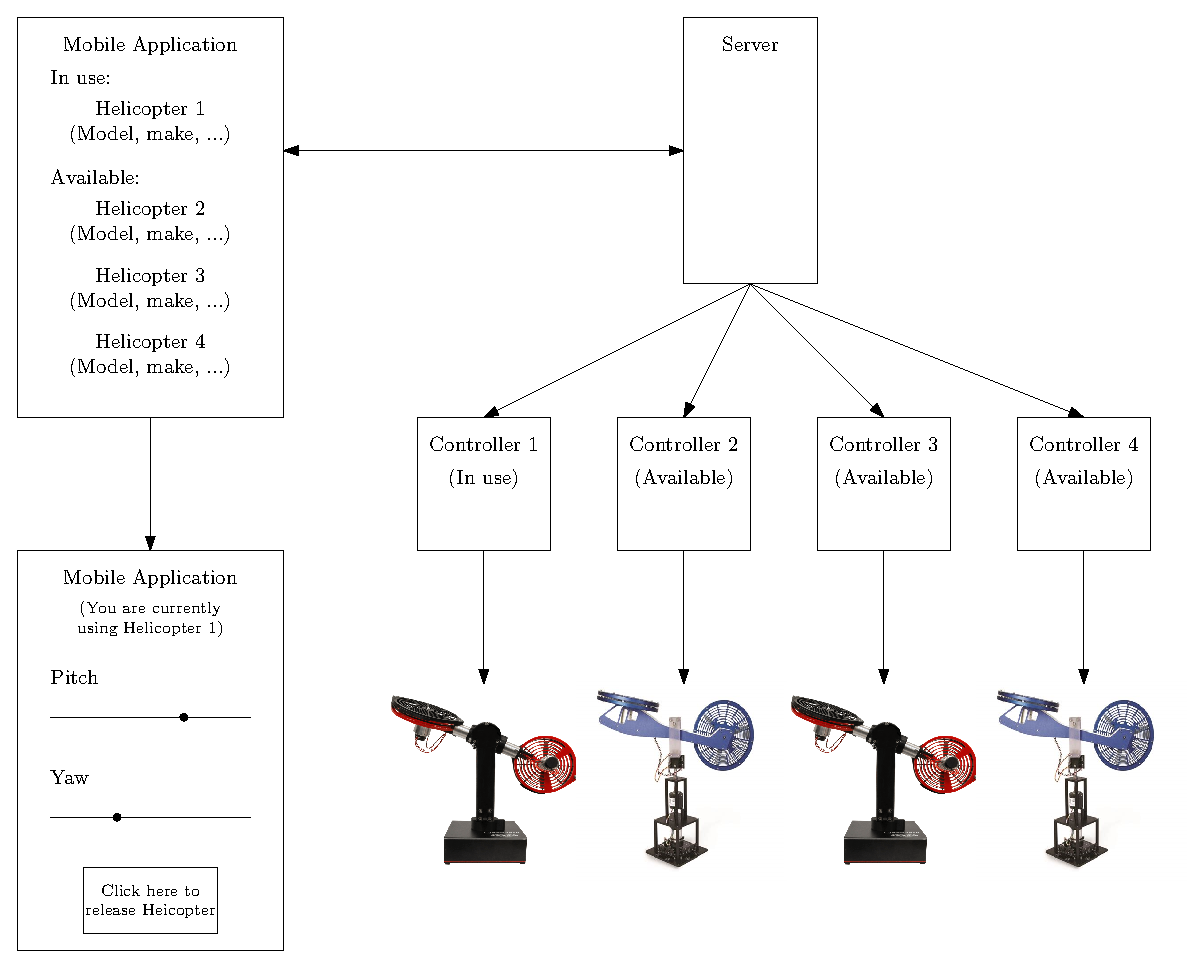
\includegraphics[width=.46\textwidth,keepaspectratio=true]{figs/ipe/smartAlg.eps}
    \label{fig:Smart_Alg}
    \caption{Smart Algorithm Server Connectivity}
\end{figure}

\subsection{Digital Compass}

\subsection{Expanded PI Control}
We had trouble implementing the PI control architecture as well as LQG on the Raspberry Pi. This may be because the integrator and the kalman filter require a fixed sampling time.  Simulink has the option to use a variable sampling time when set to continuous time.  Since the model is being loaded onto a embedded system which relies upon a fixed sampling time, this may be affected the values being outputted by these blocks.\\
To correct this issue, we recommend that future work done on this project convert the model to discrete time.  Consider \ref{eq:discreteA} and \ref{eq:discreteB} to convert the continuous model in \ref{eq:stateModel}:
\begin{equation}
\label{eq:discreteA}
    x(k+1)=\Phi x(k)+\Gamma u(k)
\end{equation}
\begin{equation}
\label{eq:discreteB}
    y(k)=Hx(k)+Ju(k)
\end{equation}
where $T$ is the sampling time, $\Phi=e^{AT}$, and $\Gamma=\int_0^T e^{A\eta} d\eta B$.
%----------------------------------------------------------------------



%%% Local Variables:
%%% mode: latex
%%% TeX-master: "../finalReport"
%%% End:
